
Instructional Design (ID) is the systematic design of effective learning experiences.
While its history stretches back into the 1940s, there are few reported cases of its formal use in Computer Science Education.
The purpose of this paper is to examine the similarities between a typical model for ID and standard software development processes.
While this equivalence between SE and ID is not novel to us~\citep{east2004applying}, we are surprised at how little literature there is within the CS community that makes this observation.
We feel that there is room for more through examination of this relationship.
This discussion is also meant to serve as an approachable introduction to ID for CS Educators who seek practical techniques for making improvements to their teaching practices.

It is our hope that readers will adopt or be influenced by ID techniques, leading them to approach their courses with the same rigor that they apply to software development.
The primary audience for this paper are educators and educational researchers specifically in Computer Science.
We use comparisons to Software Engineering as justification for the value of these practices as a design methodology, and also a way to make the material more approachable for those who are already know about SE.
Just as software development is improved by adopting various software engineering principles, instruction at all levels can benefit from the formal methods of ID.
This is true whether these methods (ID or SE) are applied strictly or just used as guiding principles.
Whether called on to teach completely new material, or improving an existing course, ID can provide a systematic process for improvement.

This paper begins with an introduction to ID.
We then present some fast and simple ways that educators can integrate principles of Instructional Design into their teaching practice. 
This is followed by a more holistic walk-through of formal instructional design methods, drawing comparisons with formal methods of software engineering.
We review the benefits and costs of applying ID methods, and then finish with a look at our own experiences and prior related research. 


\section{A Brief Introduction to Instructional Design}



\section{Practical Techniques of Instructional Design}

We encourage incremental adoption of ID best practices by CS instructors.
This approach recognizes the time pressures faced by practicing instructors who rarely have the opportunity for wholesale course redesign or radical change in their overall teaching practices.
However, through targeted adoption of specific best practices, an instructor can begin to take advantage of the improvements offered by ID.
The best practices adopted may differ among instructors to match what each believes will address the most challenging teaching issue they face and which may have the most beneficial impact on their students' learning.
Having experienced some success, at some point an instructor may find the opportunity for a more detailed and holistic study of ID.
In this section, we start on the path of incremental adoption by introducing a few simple principles, cast in terms of equivalent concepts from software engineering.  


\subsection{The Development Lifecycle}

Principled software development has a clear idea of a ``Life Cycle``, a structured sequence of phases to guide development.
ID is also a systematic process, partitioned into stages with a meaningful order.
An experienced software developer writes unit tests before code, and plans their architecture before writing unit tests.
Similarly, instructional designers begin developing new learning experiences by writing their assessments before their lessons, and their learning objectives before their assessments.
Novice educators should resist the urge to start making PowerPoint slide decks, just as novice software developers should resist the urge to start writing code.
Experienced developers in both cases give care and attention to processes to make sure that the end product meets expectations.
It is easy to write code or create instructional content without knowing the goal, but it rarely leads to a successful outcome.

Figure~\ref{dick-carey-overview} illustrates the process for one particular ID model.
There are many possible variations, but some activities must happen before others.
Planning activities such as writing learning objectives or analyzing the learners happen early on, actual development of assessments and lessons happens in the middle, and performing evaluations happen at the end.
Typically, ID models assume that revision and iterative development will occur, rather than a definitive end for each stage.
Just as software evolves over time -- to improve performance or in response to new requirements -- so also instructional materials are refined with use.

Writing learning objectives can seem like a painful activity that only gets done when forced by an accrediting agency or curriculum committee, but their value should not be underestimated.
Clearly laid out learning objectives are beneficial to both the developers and the learners.
It is easier for each to stay on track mentally if the goals are known.
Assessments (i.e., tests) can be matched directly against learning objectives, ensuring that the assessment is on target (measuring the intended learning) and comprehensive (covering all objectives).
This is similar to reviewing user requirements to ensure that all scenarios are covered by the planned software.
Clearly laid out assessments lead to a clear instructional strategy, since the designer knows exactly what the learners need in order to succeed.
Although this can lead to teaching-to-the-test if taken to an unhealthy extreme, it can also result in focused teaching with minimal distractions.
Finally, evaluations of the instructional experience (see Section~\ref{UnitTest}) can be done with a clear knowledge of the desired outcomes.

Although the flow of development shown in Figure~\ref{dick-carey-overview} is mostly linear, sometimes it makes sense to skip or return to another phase of development.
Perhaps while developing instructional materials, you realize that you left out a crucial learning objective that you felt was important.
Or perhaps while building your assessments, you realize you missed a key assumption about the entry skills of your learners.
It is important that the implications of a change to an already completed step flow to subsequently completed steps.
In the example of the new entry skill, you would want to ensure that your assessments now cover the skill, for instance.


\subsection{Unit Testing}
\label{UnitTest}

In SE, testing is used to measure one or more aspects of the code's quality (satisfies requirements, performs acceptably, is fault tolerant, etc.).
When we think of ``testing'' in the context of instruction, we likely think of giving tests to students.
We will treat the issue of evaluating testing instruments later.
For now, we consider that ID developers use testing to verify that students are learning, just as SE developers want to verify that a program satisfies its requirements.
Assessment of learning can happen at many different levels: in relation to a lesson, to a course, or a degree program.

If you inherited a large code-base and started committing purported bug fixes, how would you know if you fixed any bugs?
Unless you run unit tests before and after the bug fixes, it would not be possible to know whether you had made an impact.
A simple educational fact is that different students start with different initial performance levels and grow at different rates.
Comparing students' performance only at the end of the semester will let you know the level of performance of the students, but not the impact of instruction.
It is possible that the instruction added no new content or skill to the students.
For this reason, ID emphasizes the role of pre- and post- assessments as a key element of measuring student progress: the relative difference of their performances over the semester.
Learning gains can be defined as:

\[
Gains = \frac{Post - Pre}{100\% - Pre}
\]

In a major journal paper summarizing the results of the multi-year Media Computation project, Guzdial~\cite{??} suggests that they should have been measuring learning \textit{gains} instead of learning \textit{outcomes}.

\TODO{This section is too heavy-handed. CS instructors are going to resist both spending a lot of time on pre-tests, and also with using the same test (so "poisoning" the exam). This undermines our argument that instructors can make easy adoptions of useful (to THEM!!) practices.}

A proper pretest is administered before students engage with the instructional materials.
At the course level this usually means the start of the semester, and at the lesson level it means the start of the class.
The pretest should include every single question (unmodified) from the post-test, but can also include entry skill questions.
Instructors may find this surprising, but if the pre-test and post-test do not match, then the validity of the learning gains can be called into question.
An exception to this rule are questions that involve formula or rule application, which can vary in their details as long as the same intellectual skills is being assessed each time.
Entry skill questions help instructors ensure that all students entered with the expected prerequisite abilities.

Instructors may be hesitant to use pretests with their instruction.
There are arguments against doing so.
Deploying a pretest properly means doubling the amount of time spent on assessment, at the cost of time spent on lecture or other activities.
Instructors might fear that students will become anxious if given a test on material they have not been taught.
They could also fear that students' performance on the post-test could be affected by seeing the same questions on the pretest.
In the same way, beginning programmers often view developing unit tests as an unnecessary overhead to software development.

Instructional Designers argue that assessment should not be seen as a ``cost'', but as a valuable part of the learning process.
During a pretest, students get exposure to the kinds of problems they will have to solve, making clear what they are expected to do.
This is similar to how test-first development can be viewed as a powerful tool for better understanding the problem that future code is meant to solve.
Most instructors spend far longer on lecture and presentations than is needed, as will be discussed in a Section~\ref{??}.

Care must be taken when explaining the format and process of the pre-test to students, so that they are not overwhelmed.
Thus it is common to make pretests graded for completion or effort instead of correctness.
Avoiding anxiety must be balanced against leaving students complacent, since instructors need to have as clear an image of their learners as possible.
Regarding the fear that students might perform better only because they've already encountered the question, even without a pretest it is appropriate that students encounter the equivalent questions during practice opportunities (in-class activities, homework, projects, etc.).
Students should never be surprised on a post-test regarding the question content, or else the test instrument is likely flawed.

Another advantage of using a pretest is to give personalized or targeted instruction.
Identifying those students that need extra attention early on is challenging, but a pretest can identify students that need extra attention.
Of course, the chance of false positives is high, similar to how the number of failed test cases for a function does not perfectly predict how hard it will be to debug that function.
Besides targeting individual learners, the pretest can also reveal misunderstandings by a large fraction of the class.
It is possible that administering a pretest will reveal that students already have an understanding of some material, and that further instruction on that particular topic is not necessary.


\subsection{Design Patterns and Architectural Paradigms}

SE does not dictate what programming language to use, whether you should follow functional or object-oriented paradigms, or whether you need to use a long-polling architecture or a publish/subscribe architecture.
Using analysis techniques from SE might lead you to find that, for a given context, one of these designs is superior to the other for your particular application.
But there is nothing inherent in SE that favors or inhibits choosing among these tactical-level techniques.
In the same way, ID is a theory of teaching, not a theory of learning, and is compatible with a wide range of learning theories and educational strategies.

Similarly, ID does not demand a particular teaching style, although many models offer suggestions or templates on how to build individual lessons.
For instance, the Dick \& Carey Model advocates for designing lessons around Gagn\'e's Nine Learning Events, illustrated by Figure~\ref{gange-events}.
Briefly, these events include an introduction to the material, the presentation of the material, an opportunity to practice the knowledge gained, assessment of the learner, and a conclusion to promote transfer.
The plan for a developed learning experience can be compared against each of the events.
Critics of Gagn\'e's Learning Events suggest that the theory is grounded too firmly in Behavioralism, although Gagn\'e was later influenced by Cognitivist principles~\citep{molenda2002new}.
Variations on the Nine Learning Events exist that reflect a more Constructivist style, with more emphasis early on towards participation with less presentation.
Other instructional design models provide other templates for learning experiences.

\begin{figure}
\begin{footnotesize}

%\begin{tabular}{ |p{.19\textwidth} | p{.25\textwidth} | p{.45\textwidth}| }
%\hline
%\parbox[t]{5cm}{\textbf{Dick \& Carey's\\Instructional\\ Strategy}} & \parbox[t]{5cm}{\textbf{Gagn\'{e}'s Nine Events\\ of Instruction}} & %\textbf{Description} \\\hline
%  Preinstructional Activities & (1) Gain Attention & %Stimulate the learners and motivate them to engage %with the material. \\
%  & (2) Describe Objectives & Inform the learners %what they will be able to do because of the %instruction.\\\hline
%  Presentation Activities & (3) Stimulating Recall of %Prior Knowledge & Remind learners of their prior %knowledge. \\
%  & (4) Present the Material & Using text, graphics, %etc., give the instructional materials.\\\hline
%  Learner Participation & Provide Guidance & F %\\\hline
%  Assessment & F \\\hline
%  Follow-through & F \\\hline
%\end{tabular}

\begin{description}
\item[\textbf{\underline{Preinstructional Activities}}]
	\item[]
	\begin{description}
	\item[(1) Gain Attention:] Stimulate the learners and motivate them to engage with the material.
	{\setlength\itemindent{-40pt} \item[(2) Describe Objectives:] Inform the learners what they will be able to do because of the instruction.}
    \end{description}
%\noindent\rule{.75\textwidth}{0.1pt}

\item[\textbf{\underline{Presentation Activities}}]
	\item[]
    \begin{description}
	\item[(3) Stimulating Recall of Prior Knowledge:] Remind learners of their prior knowledge.
	{\setlength\itemindent{-40pt} \item[(4) Present the Material:] Using text, graphics, etc., give the instructional materials.}
    \end{description}
\item[\textbf{\underline{Learner Participation}}]
	\item[]
    \begin{description}
	\item[(5) Provide Guidance:] Give instructions on how to use the instructional materials.
	{\setlength\itemindent{-40pt} \item[(6) Elicit Performance:] Have the learners actively apply the new knowledge.}
	{\setlength\itemindent{-40pt} \item[(7) Provide Feedback:] Show the learners what they did well and poorly on.}
    \end{description}
\item[\textbf{\underline{Assessment}}]
	\item[]
    \begin{description}
	\item[(8) Assess Performance:] Evaluate the learners on their performance
    \end{description}
\item[\textbf{\underline{Follow-through}}]
	\item[]
    \begin{description}
	\item[(9) Enhance Retention/Transfer:] Generalize instruction with similar applications.
\end{description}
\end{description}
\end{footnotesize}
\caption{Dick \& Carey's Instructional Strategy Model interleaved with Gang\'{e}'s Nine Events of Instruction}
\label{gange-events}
\end{figure}

It is the job of the designer to determine when to follow patterns and when to make the hard decisions about breaking from a convention.
As software engineers, we have to become used to balancing factors beyond what we were taught in our classes -- thinking beyond space and time costs to consider impacts on security, code readability, and development time, for instance.
There is an expectation in the Dick \& Carey Model that learning experiences will begin and end with assessments (pretests and post-tests).
There are courses where this might be considered inappropriate.
Studio and design-based courses at the advanced level might not be appropriately assessed by written tests, and cannot be meaningfully assessed with anything other than the experience and end result of taking the course.
On the other end of the spectrum, introductory courses meant for younger learners may find it demotivating to incorporate serious assessment.


\subsection{Quality Assurance}

\TODO{This presentation is too abstract. Too much "what one might do". The style needs to be more immediate and direct. What specifically should an instructor start doing, that is easy and has impact? What are the simple tools to use to do IRT assessment of the test instrument? Be direct in making one or two concrete recommendations.}

Code coverage is an important part of software testing, used to measure the effectiveness of a test suite.
This metric is not perfect, but gives a rough idea of where to focus attention.
Similar techniques and methods exist for evaluating assessments and resources developed with ID.
At a high level, all instructional materials need to be evaluated with real learners to identify defects in the instructional materials.
These evaluations can range from individual sessions with learners to large field trials, and can yield varying levels of quantitative and qualitative evidence about the instruction.

However, assessments (i.e., tests) in particular can benefit from statistical analyses such as Item Response Theory to reveal inadequacies and validate the test items.
Consider what makes for a good exam.
Based on the learning objectives established during the early phases of the ID process, the most important content is selected and exam questions are created.
We hope and expect that a student will answer these questions correctly if and only if the student appropriately comprehends the corresponding content.
As a whole we then have a few evaluation criteria that we use to define a ``good test''.
\begin{itemize}
\item The class median and grade distribution looks like what we expect (e.g., a normal curve with a suitable median).
\item The median time and distribution needed to complete the test is appropriate.
\item Students appear to understand the question (it is not ambiguous or misleading).
\item Students do not complain to much (which is primarily dictated by good results on the three points above).
\end{itemize}

While these are necessary conditions for a good exam, and while most instructors already consider those features, they are not sufficient.
We also want to consider whether the exam appropriately covers the learning objectives, and whether we are getting the most meaningful feedback from the questions.

Item-Response Theory is a statistical methodology for evaluating the components of an assessment by their individual difficulty~\citep{van2013handbook,Sudol-itr}.
This paradigm can be useful for any kind of information: multiple choice, true/false, rubric-evaluated free response, etc.
The core concept is to model a function mapping the learners and items' parameters to the probability of a learners giving a correct response to an item.
In the IRT model, a learner can be modeled by their overall performance on the assessment.
Item parameters vary according to the specific function used, but generally numerically represent concepts such as the difficulty of the item, the discrimination of the item (how well it divides novices and experts), and mitigation of guesses.
The results of an IRT analysis can be further statistically assessed for reliability (e.g., through a Chi-square statistic), much like how unit tests can be assessed through code coverage analysis.

IRT is a powerful tool for identifying good and bad test items.
The information gathered can guide developers to fix and remove bad questions just as unit tests can identify incorrect code.
Particularly well-validated and reliable instruments can become Concept Inventories, suitable for wide-spread dissemination and use by other instructors.


\subsection{Documentation}

If a software developer handed you a zip file of undocumented source code, you would probably find it difficult to navigate and debug.
Being given only the presentation content for a course (typically in the form of a slide deck) might help you to develop your own instructional content, but it does not prepare you to teach the class.

Principled development of a learning experience results in a number of artifacts.
Some of these artifacts are meant for end-user learners: powerpoint slides, assignments, and assessments.
However, other forms of documentation are valuable to the next instructor who must teach the same course.
Following an ID process should result in useful documentation on learning objectives, learner analyses, and instructional strategy.
\TODO{Concretely, what form would this take?}
Although students never see this information, it provides crucial context for other adopters.
Documentation should ideally occur at every step in the ID process.

Programmers document code not just for other people, but also for themselves.
Have you ever reviewed older course materials that you created, and were unable to understand why you made a particular decision?
Have you ever looked at a presentation slide and could not remember what the point was?
Commenting your learning resources is just as valuable as commenting code.
Because of the time scale, large instructional design projects (e.g., a semester-long course) should be commented along the way, rather than planning on documenting at the end.

Organizing documentation artifacts can be a struggle, especially with multiple instructors collaborating to develop a course.
Discipline is required throughout the lifetime of the instructional design process.
Taking advantage of version control software such as Git can make it easier later to review the changes made to a course, to distribute materials, and even push and pull content from external adopters.

Following the complete, formal model of ID is a self-documenting process.
In the first steps of the Dick \& Carey model, for instance, you must explicitly notate the objectives, learners, and environment.
This documentation is not meant for the learners (although sharing objectives has benefits), rather is meant for the designer and future implementors.
This information is helpful in determining if a curriculum matches its needs, and whether basic assumptions about the learners were correct.
Later in the process, the Instructional Strategy should be detailed as a series of steps with annotated comments, explaining possible confusions, divergences, and so on.
The assessment instruments and practice questions are valuable to keep track of and reuse, but must be treated more carefully -- general propagation of tests could make it easier for cheating to occur.
%Compare the security needed for assessments and practice items with the secret keys or database data for applications; selectively release the relevant details to trusted parties, and document structure and mocked examples for the public.
The instructional materials themselves are usually less guarded, but decisions must be made about storing source vs generated materials (e.g., PowerPoint slides vs. PDF, comparable to source code files vs. compiled binaries).
Finally, the results of any evaluations should included along with the process used to collect those results, and notes with the decisions of the process.
\TODO{I do not understand the previous sentence. What do you mean by results of evaluation? Surely not the test scores for students. What decisions need to be noted?}
For each of these artifacts, revisions (and justifications for those revisions) should be captured.
If confusing or seemingly-arbitrary decisions are not explained, implementors run the risk of second-guessing down the line, and may attempt changes that have been previously ruled out.


\section{A Formal Model for Instructional Design}

\TODO{This entire section just makes my eyes glaze over. Do we need this at all? If so, can we cut down by a factor of 2 or 3? What are we really trying to accomplish? As written, its not going to motivate anyone to do this stuff. It reads like heavy-handed software engineering process bureaucracy that everyone ignores.}

In this section, we describe each phase of the Dick \& Carey model in more detail, following the order shown in Figure~\ref{dick-carey-overview}.
For each phase, we contextualize the description with examples and note related techniques from SE.
The goal of this section is to give practitioners a more detailed overview for using an example ID model.
For more in-depth reading, we
recommend~\citep{dick2005systematic,gagne2005principles}.

The examples used in this section are drawn from our own experiences using ID to improve our teaching.
We refer to two major scenarios, meant as guiding examples and context to give a clearer picture as to how ID is conducted.
\vspace{-\medskipamount}
 
\begin{enumerate}
\item Improvements made to a university-level, semester-long course on Computational Thinking for non-majors.
By the time the authors started applying ID techniques to improve the course, it had already been created and offered several times.
\item The creation of a high school level, week-long summer workshop on Computer Science.
The authors had great freedom to create and establish curricula, although we were under severe time and resource constraints to develop the materials.
\end{enumerate}


\subsection{ (1/9) Identify the Instructional Goals}
\label{IdentifyGoals}

The first step in the Dick \& Carey Model is to identify the instructional goal(s) that you want to accomplish.
This is similar to the SE concept of requirements analysis, the development of high-level, measurable-goals.
Critically, the goal does not describe anything about how the instructor will teach the material -- only what learners are expected to know and are able to do at the end of the instructional experience (working like an ADT).
This goal can come from a variety of sources, either top-down or bottom-up.
For instance, the four core learning objectives for our Computational Thinking course came from a university initiative, although it was up to the course instructors to decompose these objectives into finer-grained objectives.
Alternatively, these goals might be determined completely by the instructor, as with our Computer Science workshop.
Many professional organizations and colleges establish objectives according to a national or discipline-wide agenda, such as the Computer Science Curricula project~\citep{CS2013}.
Goals can also come from a specific, perceived gap in learners' existing ability.
In the Computational Thinking course, new learning objectives were incorporated about naming variables in response to students' struggles with understanding their mechanical rules.

In the full Dick \& Carey model, a \textit{Needs Assessment} is conducted to determine if instruction is truly needed.
For instance, instead of teaching employees how to use complex software, the user interface of the software could be streamlined instead.
In our Computational Thinking course, students were struggling with the IDE.
Instead of better training the students, a simpler IDE was chosen instead.
Because ID can be a time- and energy-consuming process, it can be valuable to find evidence (either quantitative or qualitative) of the need for instruction to better focus resources.

A complete goal statement should describe:
\vspace{-\medskipamount}

\begin{enumerate}
\item The learners
\item The performance context
\item The action that learners should be able to do in the performance context.
\item The tools that are available to the learners in the performance context.
\end{enumerate}
A common misstep in writing an instructional goal is to create a \textit{fuzzy goal}, usually one that describes an abstract, unobservable outcome using verbs such as ``appreciate'' or ``know''.
To correct a fuzzy goal, the designer should begin by writing down the goal.
Then, they list examples of what people do to demonstrate that they have achieved this goal.
The designer can use this demonstration-oriented list to iteratively develop more concrete goals that will lead to observable outcomes.

In the Computational Thinking course, we wanted students to better understand variables and program state.
The instructors and teaching assistants of the course repeatedly mentioned this as one of the weakest areas for students, despite being one of the most important concepts.
Many students struggled to write basic programs because of their inadequate understanding of how to use variables.
Although there were no assessments at this point that could provide definitive evidence, the questions from office hours and one-on-one sessions made the need clear.
The goal statement created for this learning objective reads as follows:

\begin{enumerate}
\item \textbf{Learners: } An undergraduate, non-Computer Science major...
\item \textbf{Performance Context:} ... Given source code...
\item \textbf{Action} ... Will be able to identify the name, value, origin, and type of a variable at any given step within the code...
\item \textbf{Tools} ... Taking advantage of any resources provided by their IDE.
\end{enumerate}


\subsection{(2/9) Conduct Instructional Analysis}
\label{learner-and-context}

\TODO{This sounds funny. Why is it a "model"? Why not a process? Or framework?}

The next step in the model is to conduct an instructional analysis, which will spell out exactly what the successful learner will do in the performance context.
This step is also similar to the SE concept of requirements analysis, but focused on a lower-level of detail in specifying measurable goals.
Like the instructional goal, it does not describe how to teach the material, although it is easy for product-oriented thinkers to accidentally start diagramming their lesson plan instead.
The instructional analysis first requires the designer to classify the goal statement based on the the kind of learning it requires.
Then, the designer identifies and organizes the \emph{subskills} involved in the skill being learned, and places them into an Instructional Analysis Diagram.

Dick \& Carey describe four learning outcomes, based on the work by Gagn\'{e}.

\textbf{Verbal Information} requires the simplest form of learning: it represents simple, declarative knowledge to be memorized and recalled (e.g., ``What is the worst-case runtime of the major sorting algorithms?'').
Little presentation is usually needed for verbal information, although students may find it useful to practice such material.

\textbf{Intellectual Skills} are more complicated problem-solving tasks that demand some level of deeper cognition (e.g., ``Write an algorithm to sort a list of numbers.''). 
Many types of knowledge in Computer Science require intellectual skills, but range greatly in complexity.

\textbf{Psychomotor Skills} are much rarer in Computer Science, describing the coordination of mental and physical activity (e.g., ``Type the alphabet using a keyboard'').

\textbf{Attitudes} is the fourth type, describing goals where the learner makes a choice (e.g., ``Choose to persevere in the face of segfaults'').
Computing education is often concerned with improving students' attitudes towards computing, leading to choices of learning further material, taking more courses, or choosing to interact with the computing community.

\textbf{Cognitive Strategies} was identified by Gagn\'{e} as a fifth domain, but can also be seen as a particularly ill-structured form of intellectual skills.
This might include more complex activities such as debugging or time-management planning.

Readers familiar with Bloom's Taxonomy will find these outcomes similar.
Mappings exist between these lists, suggesting their rough equivalence.
In both the Computational Thinking course and the Computer Science workshop, many different kinds of learning outcomes are necessary: verbal information related to basic facts of computing, intellectual skills related to the nature of programming, and even attitudes related to fostering domain identification in Computer Science.

The instructional goal of teaching variable tracing
(introduced in Section~\ref{IdentifyGoals}) is best classified as an intellectual skill, and Figure~\ref{fig-sa} is an abridged version of the Instructional Analysis Diagram created for the goal.\TODO{What makes it "abridged"? Do you mean that it is incomplete because not all of the skills are spelled out? If so, incomplete or partial would be better words. But why not give the complete picture (hopefully one that you really created for the course).}
It begins on the left with a high-level goal, which is broken down into a sequence of simpler steps (defining the variables, tracing the variables, etc.).
In turn, each of those skills is broken down further; in the case of defining variables, this involves identifying the names of the present variables, and then identifying how they were created.
Both of these subskills requires declarative knowledge to perform, which are written as leaf nodes.

\begin{figure*}
\begin{center}
	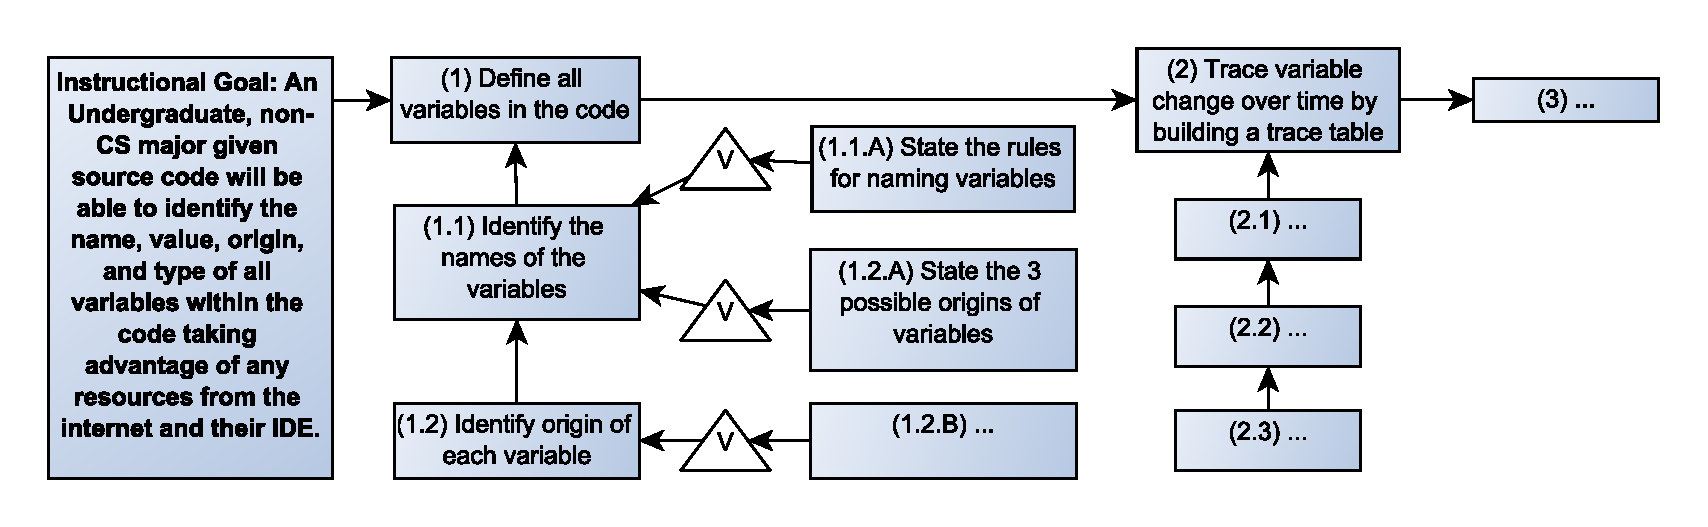
\includegraphics[width=\linewidth]{images/ia_simple}
\end{center}
\vspace{-\bigskipamount}
\caption{Partial Skill Analysis Diagram}
\label{fig-sa}
\end{figure*}

Once the goal is classified, the instructor performs a Sub-skill Analysis to concretely describe the goal and its components. 
Identifying Intellectual Skills and Psychomotor Skills is typically straightforward, by creating a flowchart that breaks down each step into multiple levels.
Much as you would decompose the steps of a program, you will decompose the skills into increasingly simpler steps.
Unlike a programming language with defined syntax to tell you where to stop the decomposition, it is up to the designer to decide when the steps are ``small enough''.
It is also possible to have branches and cycles, as is typical for flowcharts.
Some of the basic sub-skills can be considered ``entry skills'' that the learner can be expected to already have mastered before the instruction begins.
For instance, in the Computational Thinking course, basic keyboard use (a psychomotor skill) and the ability to use the browser and desktop (intellectual skills) are expected. 
Sub-steps might also involve verbal knowledge, which is denoted with a triangular ``V'' node. \TODO{What is verbal knowledge?}
Attitudinal skills can be represented as a skill that the behavior in the goal is most akin to, and elicit students to demonstrate that behavior.
\TODO{Rewrite, this sentence, I don't understand it.}

\subsection{(3/9) Conduct Learner and Context Analysis}

In the next phase, the designer identifies properties about the learners, the learning context, and the performance context. The SE equivalent is Human Factor Analysis.
Dick \& Carey suggest eight factors for understanding your learners:
\begin{enumerate}
\item their entry skills (the previously described abilities relevant to instruction),
\item their prior knowledge of the topic  area,
\item their attitudes toward content and potential delivery system (e.g., whether they prefer web-based or in-person instruction),
\item their general academic motivation,
\item their educational and ability levels,
\item their general learning preferences,
\item their attitudes toward the organization giving the instruction, and
\item group characteristics (e.g., is the group of learners heterogenous or homogenous?).
\end{enumerate}
Often the designer will intuitively know much of this information.
For some factors, it is necessary to gather information through surveys and interviews.
It is possible that this information cannot be collected until the course has already started, such as through a pre-test, or might not be collectible at all.
Designers should plan accordingly to collect the most meaningful data possible and make reasonable inferences where they can not.

In our Computational Thinking course, it was difficult to characterize the average learner and their performance context.
Students enter the course with limited prior experience with computation and, in many cases, low self-efficacy.
They can be expected to have entry skills related to basic computer use (e.g., keyboarding, browser usage), but even these are varied.
In this case, it is helpful to know the distribution of the learners' characteristics, including what ``typical'' learners look like, and also what kinds of outlier students there are.
For instance, although most students have low prior experience, every semester there have been a handful of students who have prior experience or particular aptitude for computing, making most of the material easy for them.

Conducting the performance and learning context analysis is a simpler task.
The four criteria for the performance context are:
\begin{enumerate}
\item what supervisor support is present,
\TODO{What do you mean by supervisor?}
\item physical aspects of the site (e.g., tools, facilities, etc. that are available on the site),
\item social aspects of the site (e.g., coworkers, underlings, etc. that are available on the site), \TODO{Whose coworkers and underlings?} and
\item relevance of skills to the workplace (described as a ``reality check'' by Dick \& Carey -- how will students use what they learn?).
\end{enumerate}
There are four similar criteria for the learner context:
\begin{enumerate}
\item compatibility of site with instructional requirements,
\item adaptability of site to emulate the expected work space,
\item adaptability of delivery approaches, and
\item learning site constraints.
\end{enumerate}
The reader might note a strong emphasis on the concept of a workplace, which stems from ID's widespread use in industry.
You could alternatively consider the performance context within a more abstract environment.

It might be impossible to consider any kind of ``typical'' performance context, if you are dealing with sufficiently diverse learners.
In the Computational Thinking course, for example, we deal with students from many different disciplines and with many career paths.
In the Computer Science workshop, the performance context is even more nebulous, since the goal was to simply give an introduction to the material without attempting to shape students for a particular career.
For upper-level in-major courses, or for more practical material, it becomes more valuable to consider the performance context.
For instance, when teaching a senior-level software engineering course, you might want to closely model the kinds of environments commonly encountered in industry settings.

When conducting a learner and context analysis, we recommend to identify the most salient features and not worry about exhaustively modeling learners.
In particular in Computer Science, we are often most concerned with prior knowledge and motivational factors such as self-efficacy, as opposed to students' preferences for a particular learning delivery system.
However, it is up to the instructional designer to decide what is relevant and not relevant to their process.
Our complete learner and context analysis \TODO{for what?} is available in the appendix \TODO{Do this}, arranged in tabular form for convenience, and may serve as an example of questions to consider when conducting such an analysis.


\subsection{(4/9) Write Performance Objectives}

Performance objectives, also known as behavioral objectives, establish clear and precise goals for learners, similar to the detailed specifications written in the final phase of requirements analysis.
Performance objectives are structured and rigorous, and are helpful for keeping the development process grounded and on-track.
Additionally, good objectives lead naturally to assessment instruments and lesson plans, simplifying later design steps. This is similar to how high-level program design specifications can lead immediately to implementing methods or functions.
If the objectives are used as part of the instructional materials, it is even possible that students can directly benefit from them.
Some studies have found that simply stating clear learning objectives to learners can improve their understanding and aid their cognitive strategies~\citep{torrance2007assessment}. 

Writing performance objectives is a simple, but somewhat repetitive, process.
For every skill and subskill, the designer defines three parts of a performance objective:
\begin{enumerate}
\item the conditions under which the learner will perform,
\item the behavior that they should exhibit, and
\item the criteria that they will be judged against.
\end{enumerate}
Objectives are specific and detailed, avoiding language that applies equally to any objective.
Furthermore, they use verbs that describe an observable action, rather than unobservables such as ``know'' and ``understand''.
If you cannot collect observable evidence for an objective, thenb the objective serves no purpose.
When iterating through the subskills, you can start with the instructional goal and proceed in a depth-first exploration of the instructional diagram, creating an objective for each node.

In our example of tracing variables in the Computational Thinking course, a concrete terminal performance objective for the instructional goal might be:

\begin{enumerate}
\item \textbf{Conditions: } Given some source code in python and access to resources from the internet...
\item \textbf{Behavior: } ... learners will list the name and origin and trace the value and type of all the properties ...
\item \textbf{Criteria: } ... for every variable in the code
\end{enumerate}

\TODO{Check this wording for the "Behavior" clause above. It does not really make sense to me.}

Alternatively, consider node 1.1.A, ``State the rules for naming variables'':
 
 \begin{enumerate}
\item \textbf{Conditions} Given some source code in python...
\item \textbf{Behavior} ... learners will state the rules for naming properties...
\item \textbf{Criteria} ... in their entirety.
 \end{enumerate}

\TODO{This example does not really make sense. First, why the switch from variables to properties? What are you interested in? Then, are you after a proficiency with identifying something about variables in some code, or some (abstract) knowledge about the rules for how variables work? There seems to be confusion here about which goal you are after.}

An experienced educator has probably had an unpleasant encounter with goal and objective writing while dealing with accreditation processes.
We encourage, as always, to consider the trade-offs in the process and the product.
When done correctly, ID should never get in the way of designers, but serve as a tool, just as SE principles should help the development process instead of hindering it.
Performance objectives can and should be powerful tools for organizing the course content, especially when collaborating or disseminating results.


\subsection{(5/9) Develop Assessment Instruments}

\TODO{This section is somewhat demotivating. Most instructors will not buy into preparing practice exams, let alone pre-tests.}

Software testing methodologies such as unit testing are a valuable tool in SE, helping developers to rapidly identify problems and be assured that their implementation matches the specifications as their codebase evolves.
Developing assessment instruments for students' learning is the ID equivalent.
Much like test-driven development, the Dick \& Carey model and other modern models often advocate developing assessments prior to designing and developing course materials.
By "assessments" we refer to both large exams and short quizzes, depending on the time scale of the learning experience (e.g., an individual lesson, a unit, an entire course).

There are four kinds of assessments in the Dick \& Carey Model, roughly partitioned by time.
We have already discussed the pre- and post-tests, which are given at the beginning and the end of the learning experience, respectively.
There are also practice assessments, which are meant to be used after a student has received some amount of instruction but before the post-test.
Ideally these three instruments are aligned -- whatever is on the pretest shows up on the practice test, and whatever is on the practice test is included in the post-test.
The only exception is for questions that involve application of formula, which can vary the specific values used.
\TODO{This phrasing is awkward! And this is not the first place that this comes up. You are trying to talk about a parameterized problem instance, observing that its the problem type that is learned, not the parameters. Define it this way earlier, and use this terminology where appropriate.}
The more closely the pretest and posttest are aligned, the more confident the designer can be that they successfully measured the change in their learners' knowledge.

Another type of assessment is the entry skills test, which is usually combined with the pre-test.
These questions are meant to confirm the expected prior knowledge of the learners.
Ideally, every student will achieve a perfect grade on entry skills questions.

There are many different question types.
Multiple choice and true/false are advantageous because they are easy to grade, while questions where students create or synthesize knowledge are more difficult to assess.
Essay questions are opportunities to gather more in-depth knowledge about students' understanding of a concept.
Short answer and fill-in-the-blank can be a midpoint between these extremes.
For further information on developing assessments following classical forms, we refer the reader to~\cite{nitko2001educational}.

Some forms of assessment that are relatively unique to Computer Science.
Students can be tasked with tracing code, predicting output, or writing and testing programs.
Although many disciplines have portfolio reviews, Computer Science in particular can benefit from code reviews and having students describe and critique their generated computing artifacts.
When choosing assessments, carefully consider the trade offs between the potential depth of the students' responses, the expense of grading, and the cost of developing the assessment.

\TODO{The prior two paragraphs do not tell anyone anything that they don't already know. They merely list some question and assessment types that everyone commonly uses. This has nothing really to do with the process of ID, nor does it provide any directives toward applying (simple) ID to what instructors do. Probably can just drop them.}

When designing the lesson on tracing variables for the Computational Thinking class, our main performance objective was assessed by having students trace out variables' type and value over time.
However, tracing execution is a high-level intellectual skill that involves a number of less complex skills and verbal knowledge. \TODO{What do you mean by "verbal knowledge"?}
When you trace a program, you must be able to identify all of the variables in the code and, by extension, you should know the rules for how variables are named and positioned within code.
Each of these subordinate skills should be represented by performance objectives and assessed, similar to how functions and helper functions must be unit tested, even though they might have only a small role in a large application.
For instance, to assess the recalling of variable naming rules, students were given a multiple-multiple choice question \TODO{Is "multiple-multiple" a typo? Or did you mean it?} to select all of the valid variable names.
Later evaluation revealed that, prior to instruction, students had poor performance on this subskill, which might have been unclear if the subskill had not be been tested directly.
\TODO{Why this clause "later evaluation revealed"? This sentence is hard to understand what really went on. It probably deserves to be unpacked to better explain what the process was. Also, for this example to be good, reader needs to understand how it was the ID process that caught the problem, rather than a fortunate observation by the instructors.}

According to the Dick \& Carey model, designing assessment instruments happens prior to deciding the expected delivery mechanism of the instruction.
However, it is unwise not to consider of the constraints of the learning environment.
In particular, if a digital assessment is planned, then there should be concerns about what resources students will have access to, what proctoring will be necessary, and what the affordances of the platform are.


\subsection{(6/9) Develop Instructional Strategy}

The instructional strategy is a high-level plan for the instructor to use when deploying instructional materials. 
Developing an instructional strategy is equivalent to developing an architecture diagram or otherwise formally planning out the architecture of a program.
The Dick \& Carey model suggests five components to consider when developing a strategy, as seen in Figure~\ref{gange-events}: the pre-instructional activities, presentation activities, participation activities, assessments, and follow-through activities.

The first task when developing an instructional strategy is to sequence and cluster the relevant performance objectives, much as you would build sequence or component diagrams.
The goal is to build a progression that learners can follow naturally and group logically connected performance objectives.
In some cases, this sequence will match the order of the objectives taken from the instructional diagram, and the clusters will be self-evidently distinctive.
However, this is an opportunity to use pedagogical content knowledge to recognize that some information, despite being distinct, is more easily understood in the context of other information.
For example, in the context of designing an instructional strategy to teach a series of sorting algorithms, the instructional diagram might promote each algorithm being taught sequentially.
However, an instructor might decide to cluster the performance objectives related to stating the algorithms' run-time efficiencies and order this cluster \TODO{Awkward wording! Do you mean "present the content" when you say "order this cluster"? What is the cluster? I guess the problem is too much jargon. Make more plain.} before learning individual algorithms, so that their similarities and differences can be highlighted in an overview instead of disconnectedly.
Sequencing and clustering is highly situational and will be influenced by the needs and judgments of the instructional designer.

%Just as there are design patterns and programming paradigms in Software Engineering, there are well-known templates of organization for ID.
%These templates act as guides for the creation of new content, or as checklists for existing content.
%Just as the Model-View-Controller pattern suggests how to organize code to avoid certain pitfalls and avoid missing a key element, so to do models like Gagn\'e's Nine Events help designers ensure they have achieved all the necessary components of a successful learning experience.
%But just like software patterns, there are opportunities to diverge in favor of practicalities.
%\TODO{This is not satisfying. MVC does not seem to be at the level of Nine Events. And even if it is, this is much to coarse to fit with the flavor of what I think the paragraph is after. I would like to hear about ID Patterns more on the level of Visitor or Singleton.}

\TODO{Can we do anything with the analogy to design patterns? Or are we giving up on this?}

Figure~\ref{gange-events} catagorizes Gagn\'e's Nine Learning Events~\citep{gagne1985conditions} into the five components of a learning experience according to Dick \& Carey.
This model is adaptable to different instructional styles and can respond to different learning theories.
For example, to adapt for more Constructivist approaches, one could swap Steps 4 and 6, so that students have the opportunity to engage with the materials before receiving instruction.
Whether designing constructivist or cognitivist learning experiences, it is likely that certain events will be present, no matter the order.
Note also that although this model is shown as an ordered sequence, some steps might be repeated and cycled between.
For instance, the design might suggest that the instructor give negative feedback to the learner to direct the learner to return to Step 6 until they are able to achieve some level of mastery.

\TODO{I'm sorry, but I can't bear to read this section anymore.  Skipping to Section 5.}

Dick \& Carey strongly recommend planning the Pre-instructional Activities, Assessments, and Follow-through before planning the Presentation and Participation elements, to assure optimal alignment.
They list a series of criteria to consider for each of these components.
For instance, at this point in the instructional design process, the assessments have largely been planned, and only the mechanics need to be planned. (Will it be open-note? Can students work in groups? Will it be administered on paper?)
Follow-through for the learning experience consists of devising Memory Aids (physical artifacts that students can keep to aid them later, such as a cheat-sheet showing programming syntax) and promoting transfer (e.g., by showing exactly how the learned skills can relate to their final project or future careers).

The Pre-instructional activities are a more complicated aspect to consider than Assessment and Follow-through.
First, plan to motivate the learners.
Dick \& Carey suggests using a motivational framework such as the ARCS model (gain Attention, establish Relevance, promote Confidence, and provide Satisfaction)~\citep{keller1987development}.
In Computer Science education, motivational issues often relate to anxiety and self-efficacy, but there are many other concerns.
The Learners and Context Analysis (see \ref{learner-and-context}) can be valuable for planning this stage.
Next, list the relevant learning objectives developed in the earlier phases.
Third, remind the learners of the expected Entry Skills so that they are prepared to call on those skills, or to review that material as necessary.
The Pre-instruction is often overlooked by novice designers, to the detriment of the learning experience.
Of course, Cognitive Load Theory and a mental model of the learner should also be kept in mind; many students will often skip the instructions for an assignment, no matter how well you explain them.
Still, well-written objectives and instruction can be useful for students to review as they get mired in a complicated assignment, so even if they do not read them initially, it does not mean that they will not be useful eventually.

The last two phases of the Dick \& Carey instructional strategy model are the presentation and participation components.
These components are repeatedly instantiated for all of the clustered and sequenced groups of objectives.
Notice that participation is inherent in this model, in line with modern theories of active learning.
It is already well-established in the literature that Computer Science Education benefits tremendously from such active learning techniques~\citep{mcconnell1996active}, and there are many ways to incorporate such activities.
Even a lecture has many opportunities to foster participatory discussions or for students to respond to simple questions.
In upper-level courses, where students can be expected to be more auto-didactic, there are more learning objectives, and less time available, there might be less time to commit to participatory activities.
Still, the designer should carefully consider the trade-offs and how crucial participation and feedback is to the learning process; they should probably consider giving up on learning objectives before they consider short-changing the learning experiences.

For the Computational Thinking course's learning experience on tracing variables, we planned our Presentation activities to have short videos about the material followed up by short, computer-graded quizzes that would allow students to interact with the material.
For the Computer Science workshop, different lessons were planned with very different kinds of activities.
For the second day of instruction, concerning the performance objectives about writing and debugging algorithms, students were presented with a short (10-minute) lecture on the key components of computational algorithms and then instructed to write a paper-and-pencil algorithm to sort a deck of cards.
On the third day, concerning the performance objectives about writing concrete programs, students were presented with the syntax of a simple block-based programming language, and then tasked with writing programs to accomplish simple goals (e.g., escape a maze).
Both of the participatory activities for these days were reused from other sources, a practice heavily endorsed by both instructional design and software design.


\subsection{(7/9) Develop and Select Instructional Materials}

Instructional Materials is a broad phrase that covers everything from the presentation slides to handouts to seating charts.
Developing these materials is analogous to the actual development and implementation of software, based on the architecture previously planned.
For any given materials type, there probably exist many resources to help you with their preparation.
Examples include information about strategies for activities such as designing effective lectures, creating educational videos, etc.
As the Designer moves from developing the instructional strategy to the instructional materials, they move from design to concrete development.
This decomposition of the high-level strategy into implementation mirrors the same process in software development.
Assuming care was taken in the planning phases, this should be a smooth one-way transition as the architecture naturally leads to the needed lessons.

At that point, a content delivery system is chosen based on its educational affordances and suitability for the learning experience being developed.
This delay reflects the typical role of an Instructional Designer as a \textit{consumer} of instructional technology -- they survey the available techniques and technology (e.g., traditional lecture, essay writing, websites), and choose the one that fits their need.
It is possible that Computer Science Educators can also be \textit{providers} of instructional technology, although they should consider this role very carefully.
It is always possible that the tool that they want already exists, or that an alternative teaching strategy could make it unnecessary.
There are many existing repositories of instructional materials and tools, similar to the existence of libraries in software development.

\subsection{(8/9) Conduct Formative Evaluation}

Once all of the instructional materials are completed, a Formative Evaluation should be conducted, similar to Integration Testing and End-user Testing used in Software Engineering near the end of the development life cycle.
There are three kinds of formative evaluations: 1-1, where the designer sits with three students representative of the class (i.e. one low, one medium, and one high performer); Small Group, where the materials are distributed to a collection of students and they complete them more realistically, without interaction with the designer; and Field Trial, where the instructor uses the materials in an authentic learning context (e.g., the regular classroom).
The types of evaluation to use depends on the designers' confidence in their materials and how much revision they expect they will need to make.
New materials are usually best subjected to all three phases, although this can be time-intensive and resource-intensive.

To ensure proper scientific protocol, the procedure should be planned out before the evaluation is conducted.
The use of tables and charts with specific questions can help guide the designer and make sure they gather useful data.
These questions might be about student attitudes, such as ``Did you feel confident answering when answering questions on the tests?''.
They might also be more cognitively-oriented, such as ``Did you understand what you were supposed to learn?''.

1-1 evaluation is the most personal evaluation, with the instructional designer sitting adjacent to the learner while they complete the materials.
The designer should not assist the learner, but should instead ask questions to get a sense of their thoughts and reactions.
The Small Group and Field Trials are less personal, but benefit from an increased sample size.
It is typical to include qualitative surveys in the Small Group and Field Trial evaluations in order to gather more detailed information about the motivational and practical aspects of the materials.

This is the phase of the instructional design process that can benefit from applying techniques such as Item-response theory.
When the instructor has collected sufficient data, they can apply statistical analyses to evaluate the efficacy of individual assessment items, similar to automatic measures of code coverage. 
Instructors might find that some questions were particularly poor discriminators of students' knowledge, or that they were too difficult or easy.
This information can be crucial for improving the quality of the assessment and, therefore, the rest of the material.

Figure~\ref{fe-results} shows the results for the two formative evaluations conducted for the Computational Thinking class, a 1-1 (N=3) and a Small Group (N=5).
The instruction was revised based on the results of the 1-1, before it was distributed to the Small Group.
It is important to understand that these results are not meant to show conclusive effectiveness of the instruction, but largely meant to spot weaknesses in the material.
However, the results are promising, showing large gains in the students learning from pre- to post-.
Qualitative results were also gathered during this process, revealing much more finely grained problems.
For instance, the learners in the 1-1 evaluation suggested that the audio in the videos was poor, and that they were particularly confused by the text in one of the assessment questions.
Once this material was refined, students in the Small Group trial reported a different, lesser set of problems.

\begin{figure}[ht]
\begin{center}
\begin{tabular}{l|l|c|c|c}
	Phase & Student & Pretest & Posttest & Gains\\\hline
	1-1 & \#1 & 37.8\% & 100\% & 100\%\\
	1-1 & \#2 & 51.8\% & 100\% & 100\%\\
	1-1 & \#3 & 35.7\% & 84.6\% & 76\%\\\hline
	SG & \#1 & 21.7\% & 93.3\% & 91.4\%\\
	SG & \#2 & 54.6\% & 100\% & 100\%\\
	SG & \#3 & 64.3\% & 91\% & 74.8\%\\
	SG & \#4 & 32.7\% & 80\% & 70.3\%\\
	SG & \#5 & 69.4\% & 91\% & 70.6\%\\\hline
	& \textbf{Average} & 45.9\% & 92.5\% & 86.1\%\\
	& \textbf{StdDev} & 7.5\% & 16.6\% & 9.8\%\\
\end{tabular}
\end{center}
\caption{Student Performance during Formative Evaluation (N=8)}
\label{fe-results}
\end{figure}

The Computer Science workshop was planned in a timeframe that did not allow for either 1-1 evaluations or Small Group; instead, the materials were piloted ``live'' as a Field Trial.
Although this gave much richer data, it also meant that it was impossible to revise the materials.
This is one possible explanation why the learning gain results were somewhat less favorable between these two case studies.
Of course, the nature of these two learning experiences are so different, they are essentially incomparable: the Computational Thinking unit on tracing variables was highly targeted, whereas the Computer Science workshop had much broader and high-level objectives (e.g., complicated subjects such as algorithms and abstractions) condensed into a short relatively time-span.


\subsection{Revise Instruction}

Formative Evaluation may reveal unanticipated problems with the instruction despite careful planning, similar to how careful planning and unit testing does not preclude the possibility that end-user testing may reveal inadequacies in software.
Embedded into the Dick \& Carey model is the assumption that designers will want to revise materials before moving onto more summative evaluations, expressed as a ``meta-step'' that can occur during any phase, and similar to the concept of refactoring and revising in Software Development.
Throughout the process, the designer may choose to return to an earlier phase and make revisions.
There is nothing wrong with correcting mistakes or making improvements, as long as the designer considers the downstream implications of such changes.
Deleting a performance objective, for instance, might free up a considerable amount of time to improve another performance objective, but it might also server as a prerequisite to another performance objective.
Still, iterative development is crucial no matter what kind of development is happening.
Neither software nor instruction is ever ``done'' -- it is simply ``good enough''.


\subsection{(9/9) Conduct Summative Evaluation}

When materials have reached sufficient maturity, an instructor may wish to have them disseminated for broader use.
A Summative Evaluation can be conducted by an independent third party on the validity of the objectives, instruments, and materials.
Historically, summative evaluations have shifted from comparisons of innovations (is a given instructional strategy superior to another strategy?) to demonstrations that the learners can perform in a performance context.
The dearth of concrete, monolithic performance contexts in Computer Science education can make it difficult to conduct summative evaluations.
If a lesson on the use of iteration in algorithms is developed, how can this be related to the students' future careers?
Each student may be destined for a very different path in a very different subject, and may not encounter the taught skills in any shape close to the one taught.

This case study did not involve a Summative Evaluation, as is common for many instructional design projects.
In fact, typically summative evaluation is most useful for training in industrial scenarios, rather than education in more scholarly settings.
Still, the two types of summative evaluations might have some merit if used strategically.
The first type of summative evaluation is an Expert Judgment evaluation, where an acknowledged expert evaluates the materials for fitness without interaction with the target learners.
Ideally, this expert has both content knowledge and pedagogical content knowledge.
The second type of summative evaluation is the Impact Evaluation, where the effect on the job-site is used to determine if the organizational or institutional needs have been met.
In a university setting, this might entail looking at long-term graduation results, job-placement data, or exit interviews and examinations.
Although a properly-conducted summative evaluation can provide compelling evidence for the success of instructional design, it can be very difficult and ultimately worth less than spending time on other phases or even other projects.


\section{Benefits of Instructional Design}

Instructional Design can have a number of advantages. 

\begin{description}

\item[Fault localization:]
A good instructor might be able to intuitively identify problem areas in a course.
Proper assessment measures learning gains rather than absolute knowledge, making it easier to evaluate the instructional materials.
\TODO{How do the previous two sentences relate to each other? How do either relate to the term "fault localization"?}

\item[Better Tests:]
Many instructors consider assessment as an afterthought, only deployed at the end of the course.
And often, the assessment (the test) does not do a good job by any measure.
Following ID will lead to more productive tests.
\TODO{Productive measured how?}
Using simple tools such as Item Response Theory packages can increase validity of the test and identify questions that have no use to you as an instructor.

\item[Documentation:]
When developing according to ID processes, a natural side-effect is the documentation of instruction.
This goes beyond the instructional materials to include the instructional strategy, the assessments, the learning objectives, and all other components.

\item[Easier Dissemination:]
Few courses are built from scratch.
In most cases, course replication means using another instructor's materials, or course design.
There is no explanation of the decisions that went into development of these course materials, no strategy for how to use them in a greater course context, and no basis on how to modify them for a different group of learners.
\TODO{Rewrite previous sentence.}
Compare inheriting instructional materials to inheriting a codebase. 

\item[Better Specifications:]
Research has shown that merely presenting the course objectives to the students can measurably improve their performance on assessment~\citep{torrance2007assessment}.
Seeing the exact learning objectives that they are responsible for can aid students' meta-cognitive strategies.
This also aids the transfer process.

\item[More Structured Design:]
ID provides a model instructional strategy with five key components.
Constituent \TODO{Odd word choice!! What do you mean?} in this model are opportunities for students to participate actively with materials and receive feedback.
This template becomes a useful guide for designers to build their lessons around, scaffolding the design experience.

\item[Compatibility with other techniques:]
As CS instructors grow professionally, they encounter new learning and teaching techniques to guide their decisions.
ID is a framework that is compatible with a range of popular theories, including constructivism, peer instruction, active learning, and many more.
At its heart, instructional design is an approach to developing lessons, but it only offers suggestions on where to go.
\TODO{How is this section presenting a benefit? Seems like merely an incidental observation.}

For instance, active learning is inherently suggested in the model instructional strategy; the Constructivist approach is a modification of that strategy where participation precedes content presentation.
Situated Learning Theory dictates authentic assessments where learners focus on performance of tasks rather than artificial completion of, for example, written questions; Instructional Design does not require any particular assessment tools, and would suggest simply ensuring a concrete rubric (of an appropriate open-endedness) exists for the assessment activity.

\item[More Focus on User Needs:]
In Usability Engineering, the users' needs and desires are given primacy, carefully considered before any code is written.
ID similarly recommends analysis of the learners and the environment before any instructional strategies or materials are developed.

In both Usability Engineering and ID, it can become apparent early in the analysis phase that new software or instruction is not necessary.
Using a Needs Assessment, the designer can determine if there is a performance gap that can be remedied with new materials.
In many cases, changes to the tools, management, and other factors can yield desirable results without as much work.
Of course, we expect many readers to be in learning situations where they have a clear need for instruction.

\end{description}


\section{Potential Disadvantages of Instructional Design}

Of course, there can also be hazards to the process, depending on how it is applied.


\begin{description}

\item[Over-rigorous:]

The Dick \& Carey model is a teaching model, used to train new instructional designers.
It is one of the most formal methods of instructional design, with rigorous amounts of structure and a strong sense of linearity.
\TODO{Does this mean that its not a good starter model to use for our audience?}
Although the entire model is iterative, the purest execution is intended to be done in discrete phases.
Each one of these individual phases demands extensive consideration and the elicitation of many details, some of which may feel repetitive or unnecessary for an instructor.
\TODO{You are not motivating anyone here!}
Identifying all of the learning objectives in a course can lead to a staggering amount of previously implicit information.
A highly detailed skill analysis leads to many performance objectives and triple the number of assessment instruments.
Although this is beneficial in a spirit of optimizing the course materials, it can be detrimental to an instructional designer with time and energy constraints.

As budding instructional designers improve, they are expected to apply formal methods more strategically.
In practice, many designers rely on more stream-lined models, a combination of their favorite models, or even to simply rely on their own intuitions.
This is similar to how Software Engineers develop intuitions about their development methods.

Some instructors may find that they work best by adopting principles or components of the instructional design model, rather than a whole-sale immersion.
We encourage trial runs and \TODO{Something is missing here}.

\item[Over-assessment:]
Although Instructional Design does not demand a minimum amount of assessment, it is implicit that learners will be evaluated summatively.
This is not necessarily compatible with all learning scenarios.
Younger learners in K-12 contexts may not be sufficiently motivated to participate in activities that they know will be graded.
It is up to the instructor to make decisions
Some instructors may not feel it is appropriate to give pre-tests to students, if they feel that the learners have no possibility of prior exposure and could be intimidated by such an assessment.

The nature of instructional design leads to tight, focused lessons where the materials and assessments are directly aligned.
Some may feel that the assessment materials are over-focused, leading to a "teach-to-the-test" mentality.
This might encourage negative, performance-oriented behavior in learners.
Even worse, exams carry emotional weight for students, and they may react badly if they feel test exhaustion.

\item[Over-structured:]
Much like programming, there is an element of art to teaching.
Introducing rigor can have implications for implicit and variable aspects of a lesson.
Sometimes, the best learning experiences happen organically because of a student-prompted question, or because of a serendipitous event during a demonstration.
If these are factored out because a lesson is too tightly controlled, valuable opportunities might be lost.
There is value in letting learning opportunities have space for more ad-hoc interactions between the learners and instructors.

Over-emphasis on the primary learning objectives might lead to underestimated secondary learning objectives falling by the way-side;
instructors might not consider certain topics to be important enough even though they have unrecognized down-stream importance to students' careers.
The importance of any given learning objective is subjective and fluctuates with time and the evolution of the field, so it is difficult to predict what is necessary for students down the line.
An instructor might, for instance, focus on mechanical or semantic details of a language, and completely avoid style details, leading students to have to learn this less crucial but not unimportant material on their own later.
Ideally, instructors should carefully consider what they should teach their students, but also refer to standards and the CS educational community so that they are not missing out on important outcomes.

Further, tightly focused lessons can limit students' perspective.
If the education is of a sufficient quality, they may believe that they are receiving the whole story, when the lesson is meant to only capture a slice of a bigger topic.
They may also develop misconceptions about the iterative nature of design.
Finally, there are viable concerns about ``spoon-feeding'' the material, leaving students reliant on high-quality instruction in order to learn material, when the reality is that most later learning must be self-directed.
Proper instructional design can provide learning opportunities to improve students cognitive skills and promote self-directed learning.
Further, we caution educators to not underestimate the difficulty of much computing material when attempting to guide students to become more auto-didactic; if the material is sufficiently difficult, it is better to focus on making it as accessible as possible rather than leaving them on their own.

\end{description}

\TODO{There is something wrong here that I cannot quite put my finger on. It has to do with the fact that our recommendations (especially Section 4) are guilty of some of the negatives described in this section. They universally come from overblown process, similar to overblown SE practice.}


\section{Discussion of the authors' experience with instructional design}

When applying the ID techniques to the summer workshop on Computer Science for high schoolers, a looser process was used.
Although learning objectives were produced and developed into assessments, much less attention was paid to filling out extensive charts detailing learner characteristics or exact performance objectives.
These modifications can be related to Agile design methods, with a focus on developing a prototypical product rather than exhaustively following the process.
Although the results from the evaluation of the Computer Science workshop were not as positive, they are promising for a first draft. 
However, from the designers' point of view, the best part of the results is not that they were positive (which they largely were), but that they had measurable results at all.
Subsequent iterations of the workshop can now be compared and referenced to each other, benefiting from both a pedagogical perspective and from a research perspective.


\section{Conclusions}

In this paper, we have attempted to contextualize the field of ID using SE.
We highlight quick and simple steps that instructors can use to immediately integrate ID into their own courses, give a thorough description of a complete ID process, and discuss the advantages and disadvantages of a rigorous design methodology.
We hope that Computer Science Educators will be able to apply principles of Instructional Design and related techniques like Item-Response Theory to improve their instruction.